\documentclass[conference]{IEEEtran}
\IEEEoverridecommandlockouts
% The preceding line is only needed to identify funding in the first footnote. If that is unneeded, please comment it out.
\usepackage{cite}
\usepackage{amsmath,amssymb,amsfonts}
\usepackage{algorithmic}
\usepackage{graphicx}
\usepackage{textcomp}
\usepackage{xcolor}
\def\BibTeX{{\rm B\kern-.05em{\sc i\kern-.025em b}\kern-.08em
    T\kern-.1667em\lower.7ex\hbox{E}\kern-.125emX}}
\begin{document}

\title{Semiconductor Physics Lab Report}
%\thanks{Identify applicable funding agency here. If none, delete this.}

\author{\IEEEauthorblockN{1\textsuperscript{st} Given Name Surname}
\IEEEauthorblockA{\textit{dept. name of organization (of Aff.)}}
}

\maketitle

\begin{abstract}
XXX
\end{abstract}

%\begin{IEEEkeywords}end{IEEEkeywords}

\section{Introduction}
XXX
\section{Procedure}
XXX
\subsection{Lab1: XXX}
XXX
\subsection{Lab2: XXX}
XXX
\subsection{Lab3: XXX}
XXX

\section{Results and Discussion}
XXX
\subsection{Lab1: XXX}
XXX

\begin{figure}[h]
\centering
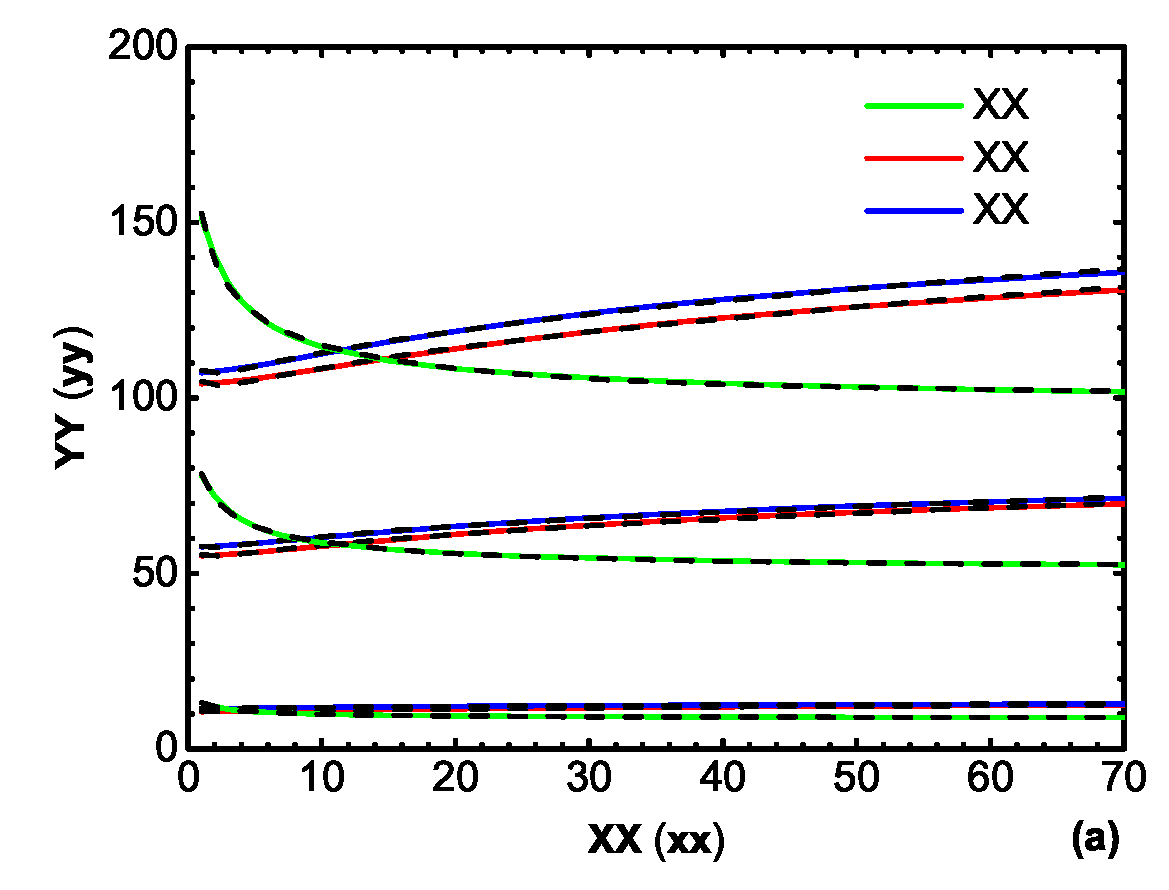
\includegraphics[width=2in]{Fig1.eps}
\caption{Schematic diagrams and coordinate system for the (a) 2D C-SJ and (b) 3D C-SJ structures.}
\label{Fig1}
\end{figure}

\subsection{Lab2: XXX}
XXX
\subsection{Lab3: XXX}
XXX

\section{Conclusions}
XXX

\section{Appendix\\
Numerical Calculation Code for Lab 1 (Relationship between Equilibrium Electron Concentration and Temperature)}
XXX


\begin{thebibliography}{00}
\bibitem{b1} G. Eason, B. Noble, and I. N. Sneddon, ``On certain integrals of Lipschitz-Hankel type involving products of Bessel functions,'' Phil. Trans. Roy. Soc. London, vol. A247, pp. 529--551, April 1955.
\bibitem{b2} J. Clerk Maxwell, A Treatise on Electricity and Magnetism, 3rd ed., vol. 2. Oxford: Clarendon, 1892, pp.68--73.
\bibitem{b3} I. S. Jacobs and C. P. Bean, ``Fine particles, thin films and exchange anisotropy,'' in Magnetism, vol. III, G. T. Rado and H. Suhl, Eds. New York: Academic, 1963, pp. 271--350.
\bibitem{b4} K. Elissa, ``Title of paper if known,'' unpublished.

\end{thebibliography}

\end{document}
